\documentclass{beamer}
\usetheme{Boadilla}
\usepackage{booktabs}
\usepackage{adjustbox}
\usefonttheme{serif}
\subtitle{Using Beamer}
\usepackage{pgffor}

\title{ \textbf{Stepscan Project}}
\subtitle{Results of Worksheet 1-3}
\date{\today}
\author{Saeed Kazemi}
\institute{ University of New Brunswick}
\usepackage{caption}

\begin{document}


%%%%%%%%%%%%%%%%%%%%%%%%%%%%%%%%%%%%%%%%%%%
%%%%%%%%%%%%%%%%%%%%%%%%%%%%%%%%%%%%%%%%%%%
\begin{frame}
\titlepage
\end{frame}


%%%%%%%%%%%%%%%%%%%%%%%%%%%%%%%%%%%%%%%%%%%
%%%%%%%%%%%%%%%%%%%%%%%%%%%%%%%%%%%%%%%%%%%
\begin{frame}
\frametitle{Outline}
\tableofcontents
\end{frame}


%%%%%%%%%%%%%%%%%%%%%%%%%%%%%%%%%%%%%%%%%%%
%%%%%%%%%%%%%%%%%%%%%%%%%%%%%%%%%%%%%%%%%%%
\section{Score Matrix}
\foreach \n in {afeatures\_simple, afeatures\_otsu, pfeatures, COAs\_otsu, COAs\_simple, COPs}{
\begin{frame}
\frametitle{Euclidean distance vs Correlation + \n-Mode-Acc}
\tiny
\begin{table}
\centering
\captionsetup{labelformat=empty}
\caption{\footnotesize The accuracy of Euclidean distance and Correlation on COP features.}
\begin{tabular}{lll}
\toprule
{} &                  Accuracy Left &                 Accuracy Right \\
\midrule
Euclidean distance &  69.33 +/- 3.79 (60.51, 76.44) &  69.26 +/- 3.49 (60.60, 75.93) \\
Correlation        &  65.45 +/- 3.13 (59.32, 71.44) &  64.61 +/- 2.83 (59.49, 70.42) \\
\bottomrule
\end{tabular}

\end{table}
\begin{table}
\centering
\captionsetup{labelformat=empty}
\caption{\footnotesize The ERR of different size of the test set.}
\label{tab:parameters condition}
\begin{tabular}{lll}
\toprule
{} &                    EER Left &                   EER Right \\
\midrule
Euclidean distance &  0.29 +/- 0.02 (0.26, 0.31) &  0.28 +/- 0.02 (0.25, 0.31) \\
Correlation        &  0.31 +/- 0.03 (0.27, 0.36) &  0.30 +/- 0.03 (0.26, 0.34) \\
\bottomrule
\end{tabular}

\end{table}

\begin{block}{\small Conditions}
    \footnotesize These results are average over the results of below conditions: min, mean and median criteria, All PCs and 95\% variances, Min-Max and z-score algorithm. 
\end{block}

\end{frame}



\begin{frame}
\centering
\frametitle{Euclidean distance vs Correlation (ROC curve)}
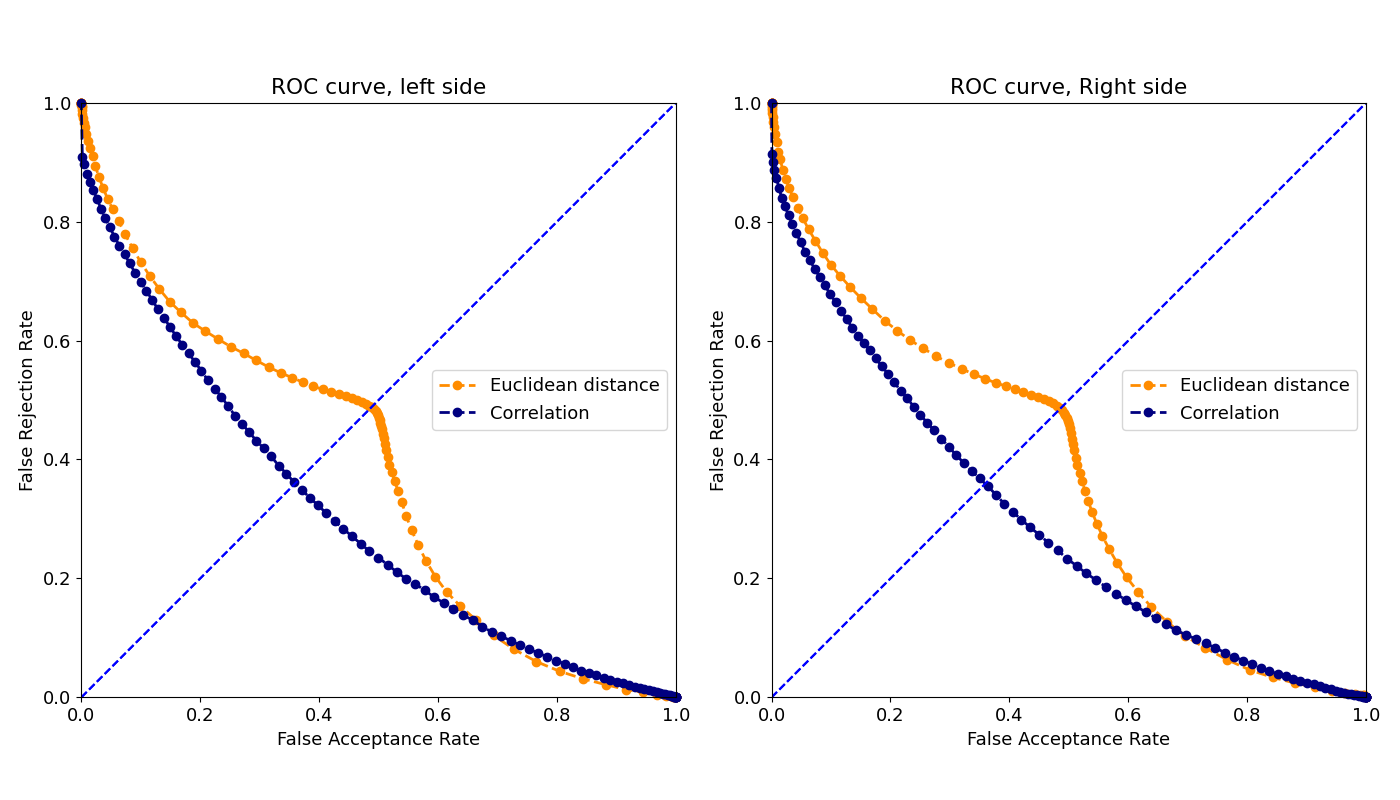
\includegraphics[scale=0.3]{Manuscripts/src/figures/pfeatures-Mode.png}
\end{frame}

}

\end{document}

